\documentclass[10pt,twocolumn,letterpaper]{article}

\usepackage{cvpr}
\usepackage[utf8]{inputenc}
\usepackage{gensymb}
\usepackage{graphicx}
\graphicspath{ {imgs/} }
\usepackage{float}

\cvprfinalcopy
\def\cvprPaperID{a1700831}


% begin of document
\begin{document}
\title{Assignment 1 - Method for Creating Mosaics by Brown and Lowe}
\author{Yuanzhong Xia\\
University of Adelaide\\
SA, Australia\\
{\tt\small a1700831@student.adelaide.edu.au}
}
\maketitle

% abstract
\begin{abstract}
This is the assignment 1 report, describing and testing a method for creating panorama from a set of small images.
The related codes are using Java binding version of OpenCV, and it contains my test codes to evaluate my hypothesis and program performance.
\end{abstract}


\section{The Problem}
The problem is to stitch many small images representing for different part of the area space into a large panorama image.
However, the small images often have lots of issues when being stitched together.
The images can have different rotations, scales, affine or projective transformations, photometric problems, moving objects and so on.

To stitch the images into a large panorama, the method must overcome most of the issues above,
and the most important thing is to make sure the panorama looks normal and edges are less noticeable.


\section{Brown and Lowe's Method}
The method is being discovered for a long time. But none of them can perform better than Brown and Lowe's method \cite{origin}.
Brown and Lowe's method can overcome the issues caused by variant orientations, zooming, and do color corrections and moving object detection to some extend.

The method is based on invariant features appearing in multiple images. If the combination of invariant features in two images match with each other,
they can be stitched together by superimposing the matching features, and vise versa, they cannot stitch images if they don't have invariant features. 

\subsection{Description}
The psedocode on the paper has already shown the outline the stitching algorithm.
Here are the more detailed description,
\begin{enumerate}
    \item
        Read all input images,
        \textit{(if the number of images is less than two, \textbf{fail} because one image does not need to be stitched.)}
    \item \label{n:e}
        Extract SIFT \cite{sift} features from all images,
    \item \label{n:k}
        Store $k$-nearest neighbor features using a k-d tree \cite{knn},
        \textit{(increase the accuracy for feature matching.)}
    \item \label{n:m}
        Match the potential images using RANSAC \cite{ransac}, and verify them using a probabilistic model;
        a feature of this method is the images can be divided as disjoint set which means small images from different scenes can be distinguished and stitched separately,
        \textit{(if the probabilistic prediction is not high enough, and there isn't any image can be stitched with this image, \textbf{fail}.)}
    \item \label{n:r}
        Reshape and align the images using bundle adjustment \cite{bm},
        \textit{(make the stitching seamless.)}
    \item \label{n:s}
        Straighten the whole panorama by simulating the centric camera and projection effect,
        \textit{(eliminate issues caused by different camera orientation.)}
    \item \label{n:g}
        Gain compensation by weighted averaging the pixels of overlapped areas,
        \textit{(remove significant stitching edges.)}
    \item \label{n:a}
        Apply multi-band blending to the final images,
        \textit{(removed overlapping effect produced by gain compensation, caused by inaccurate match.)}
    \item \label{n:o}
        Output the panorama image.
\end{enumerate}

% todo: add some numeric analysis
% todo: more on probabilistic model

\subsection{Limitation and Improvements}
In Section 9 of the original paper, Brown and Lowe put some potential future works which are the weaknesses and possible improvements for current version of the method.
\begin{itemize}
    \item
        Camera position is often moved (at slightly) when trying to take lots of photos in real cases.
        That means the image aligning cannot be finished by simple reshaping because of scene depth, shading and overlapping.
        However, Brown and Lowe's method is the kind of ``simple'' method, it uses the feature that those images are assumed to be captured by a centric camera.
        Therefore, they use a camera position detection idea to straighten the long curved image into long straight image.
        Usually, the resulting image can contain overlapping blur effects.

        Some of them can be deblurred by Bascle \textit{et al.}'s method \cite{bascle}.
        The rest of them might require 3D modeling for a perfect fix.
    \item
        Scene can also be dynamical. Moving objects like trees and birds can also affect the stitching result.
        Although multi-band blending can solve some kinds of blur effect caused by slight motion,
        it doesn't work for large motion case.

        The way to solve it might be detecting the same object, and keeping one complete copy or removing the incomplete object.
    \item
        Advanced camera modeling. This is what I firstly came out when I saw the title with ``using invariant feature''.
        The method is limited into 2D space due to using invariant features.
        In 3D space, objects might obstruct the view, and when the camera moves, the objects will distort a lot.
        Just like Fig \ref{fig:cameramotion}, the camera orientation is vertical to the horizon line on the wall, and the motion direction is parallel with the wall.
        It is very clear that the table and chair on the images distort heavily.
        
        With 3D modeling or simulating a 2D scanner, the issue can be solved.
    \item
        Color correction is also not perfect.
        Influenced by gain compensation, the overlapped area is evaluated by error rate first,
        then the gain parameters for the whole images are calculated by a quadratic objective function.
        However, the resulting image can be easily found to have abnormal colors in overlapped areas (e.g. the overlapped area is yellowing).

        One way to solve the problem mentioned in the paper is to uniforming the colors from a common source first, like sky.
        In this way, some issues caused by over exposed images can also be fixed.
\end{itemize}

\begin{figure*}
    \begin{center}
        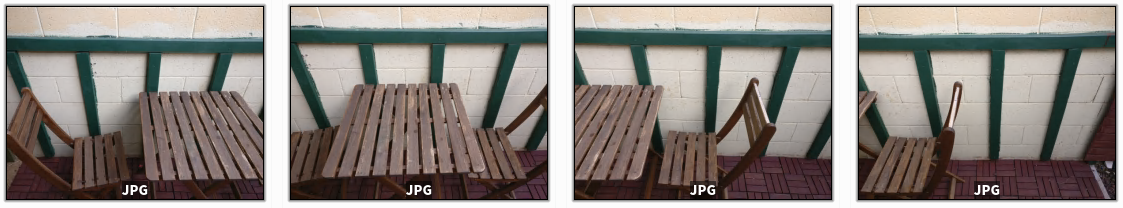
\includegraphics[width=0.9\textwidth]{horizontal_motion}
    \end{center}
    \caption{The source images are captured by horizontal moving camera, so the space projection structure is changed in every image,
    and it is impossible to match features using mentioned image matching algorithm.}
    \label{fig:cameramotion}
\end{figure*}

The weaknesses above are still current research topics, which are not easy to solve by myself. Instead, I have the following two patching extensions.

The \textbf{first} one is a more specific panorama stitching case - scanning plane information (images, documents, etc.) by moving camera.
This problem is different from the first mentioned weakness above.
The images to be stitched are in the same plane, so there are no view depth and no shading effect.
However, no matter how the photos are taken, by a centric camera or by a moving camera, the resulting images cannot look like a plane.
i.e. For local photos of a whole picture, the resulting image is expected to be like a scanned picture.

To solve this problem, the algorithm should accept another parameter ``in plane mode'',
after applying Brown and Lowe's method, the algorithm should find the rectangle outlines of the plane area
(in the resulting, it is often a curved quadrangle. (see the yellow lines in Fig \ref{fig:cml}.)
Then, reshape the final panorama to make the outline a rectangle.

\begin{figure}[t]
    \begin{center}
        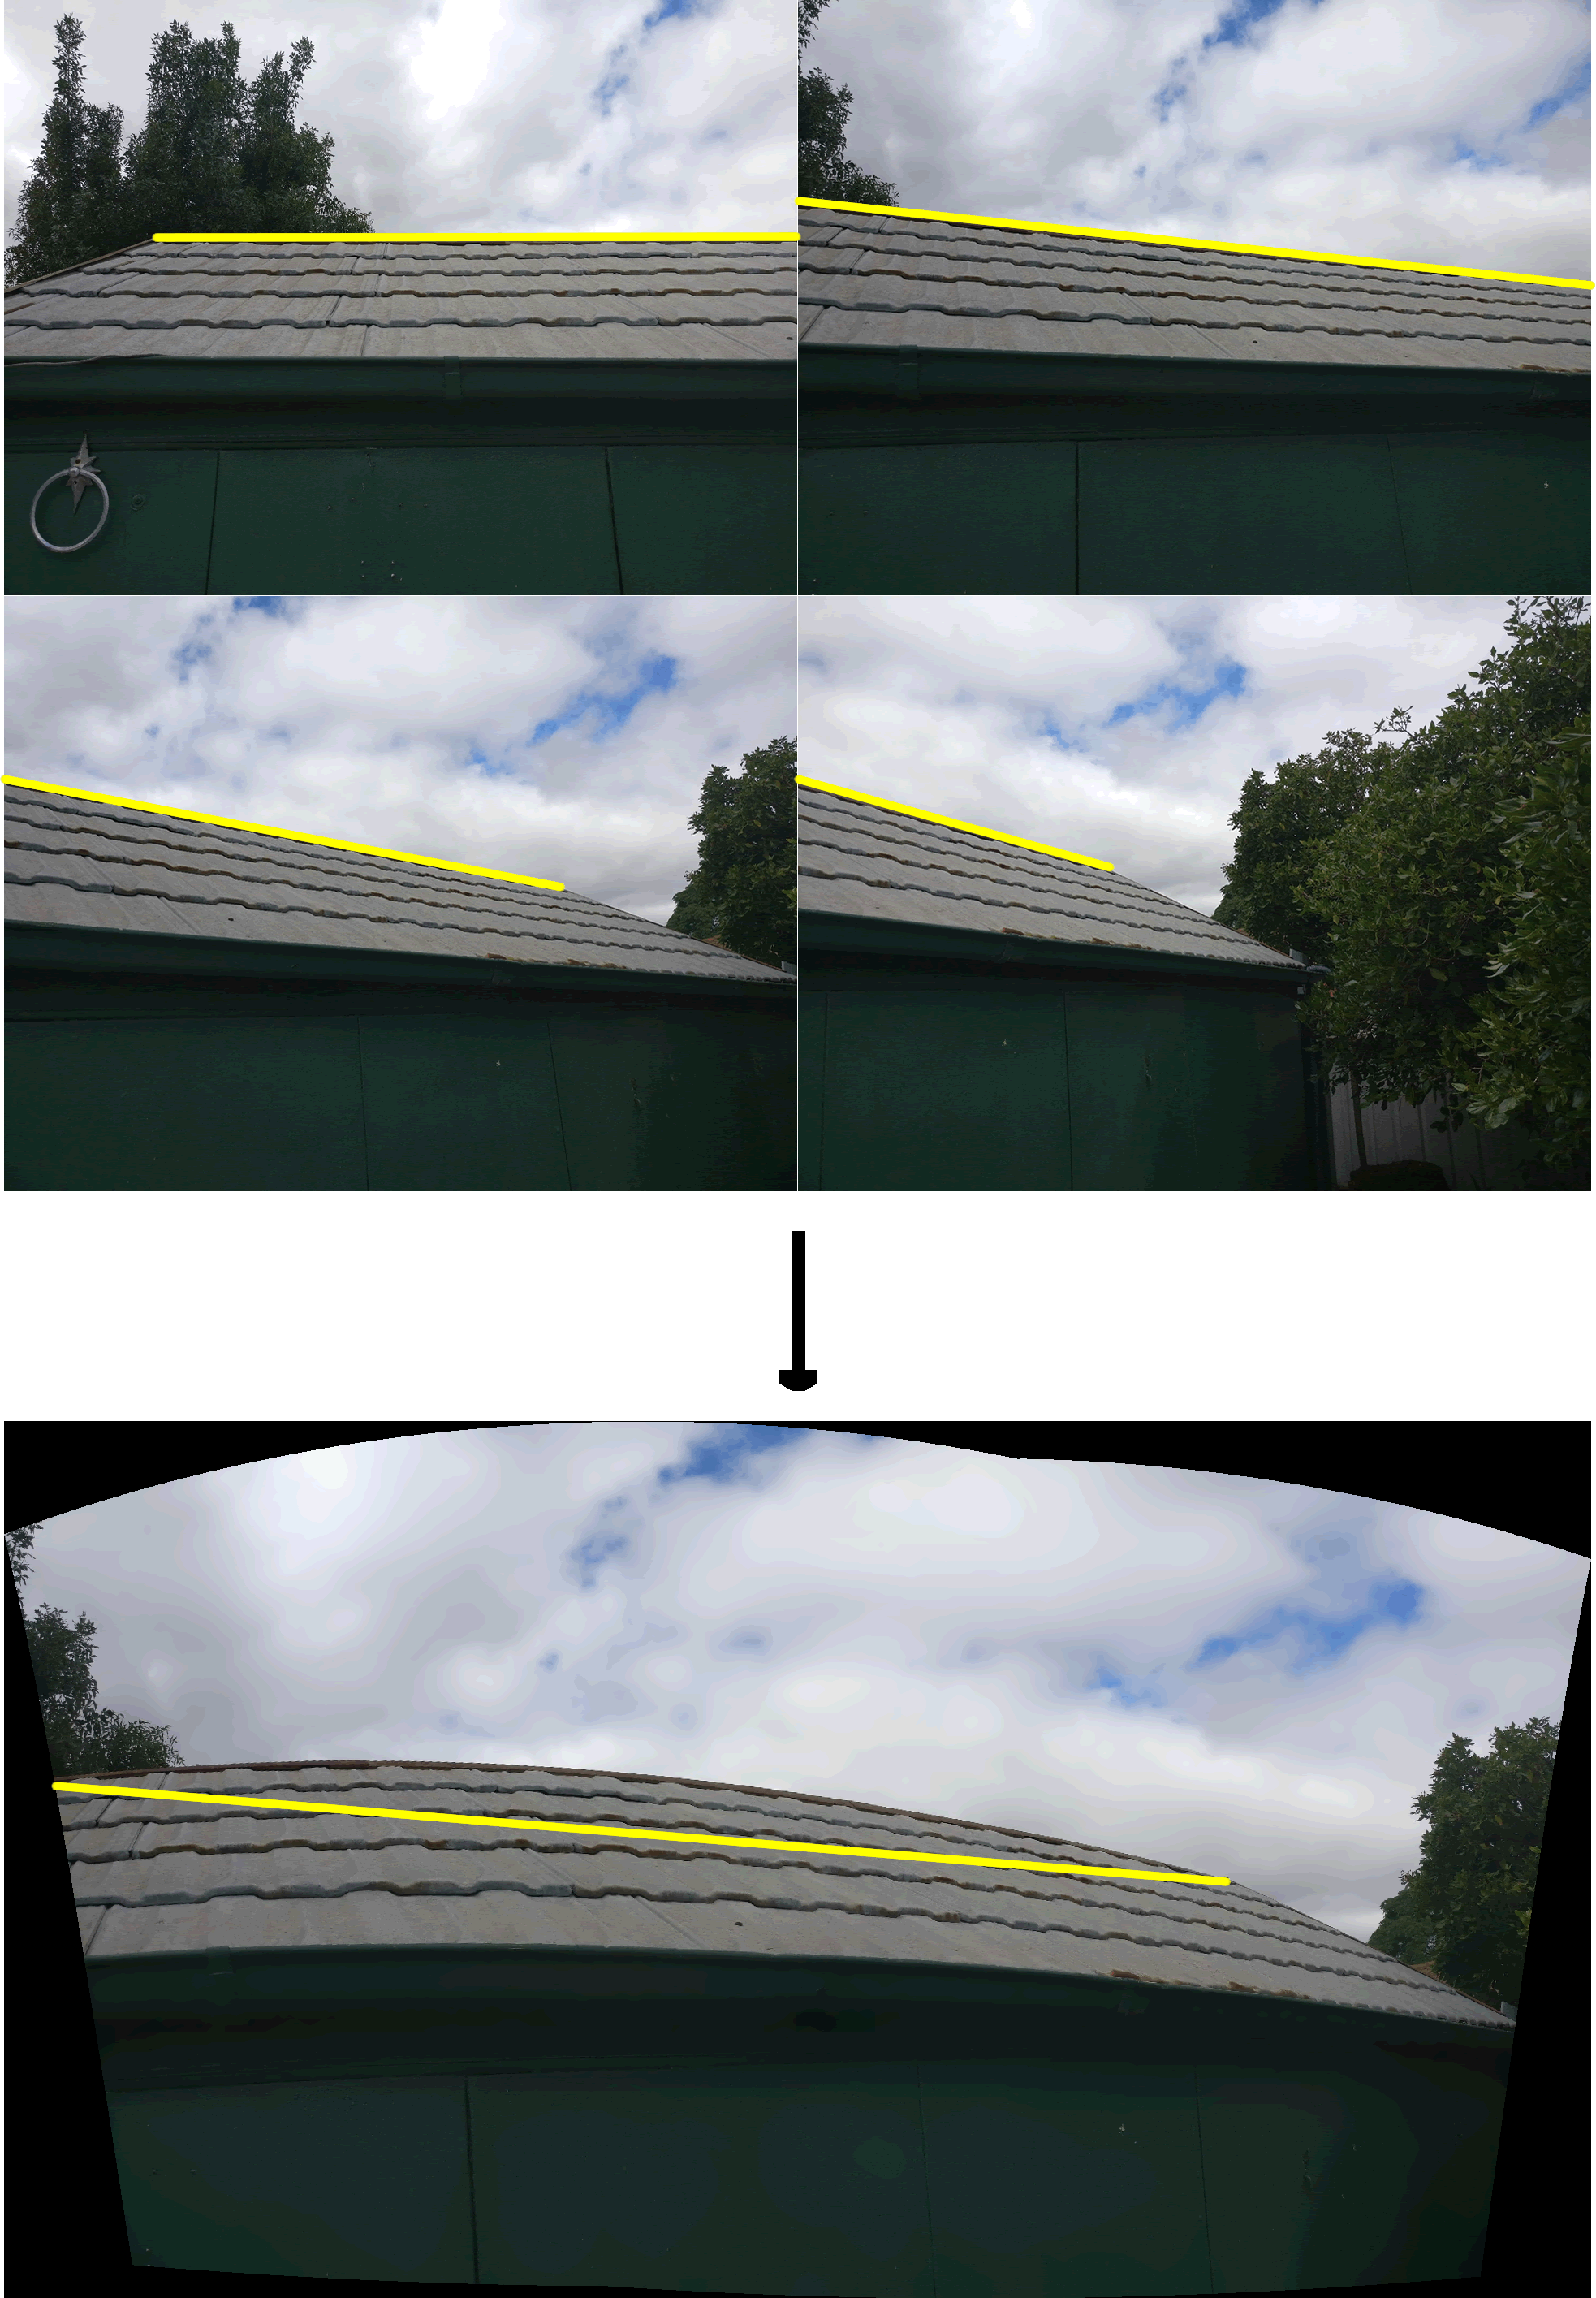
\includegraphics[width=0.9\linewidth]{line_combine}
    \end{center}
    \caption{After the stitching method, straight lines are often reshaped into curves.}
    \label{fig:cml}
\end{figure}

The \textbf{second} extension is when the image doesn't contain enough features.
Using the OpenCV implementation, if the images are very simple (like Fig. \ref{fig:pc}),
the probabilistic model will tell that the images don't have enough probabilities to match correctly.
Then, they cannot be stitched.

The optimization patching solution is to reduce the $p_{min}$ in Formula (12) in the original paper when there is no more potential matchable images.

\begin{figure}[t]
    \begin{center}
        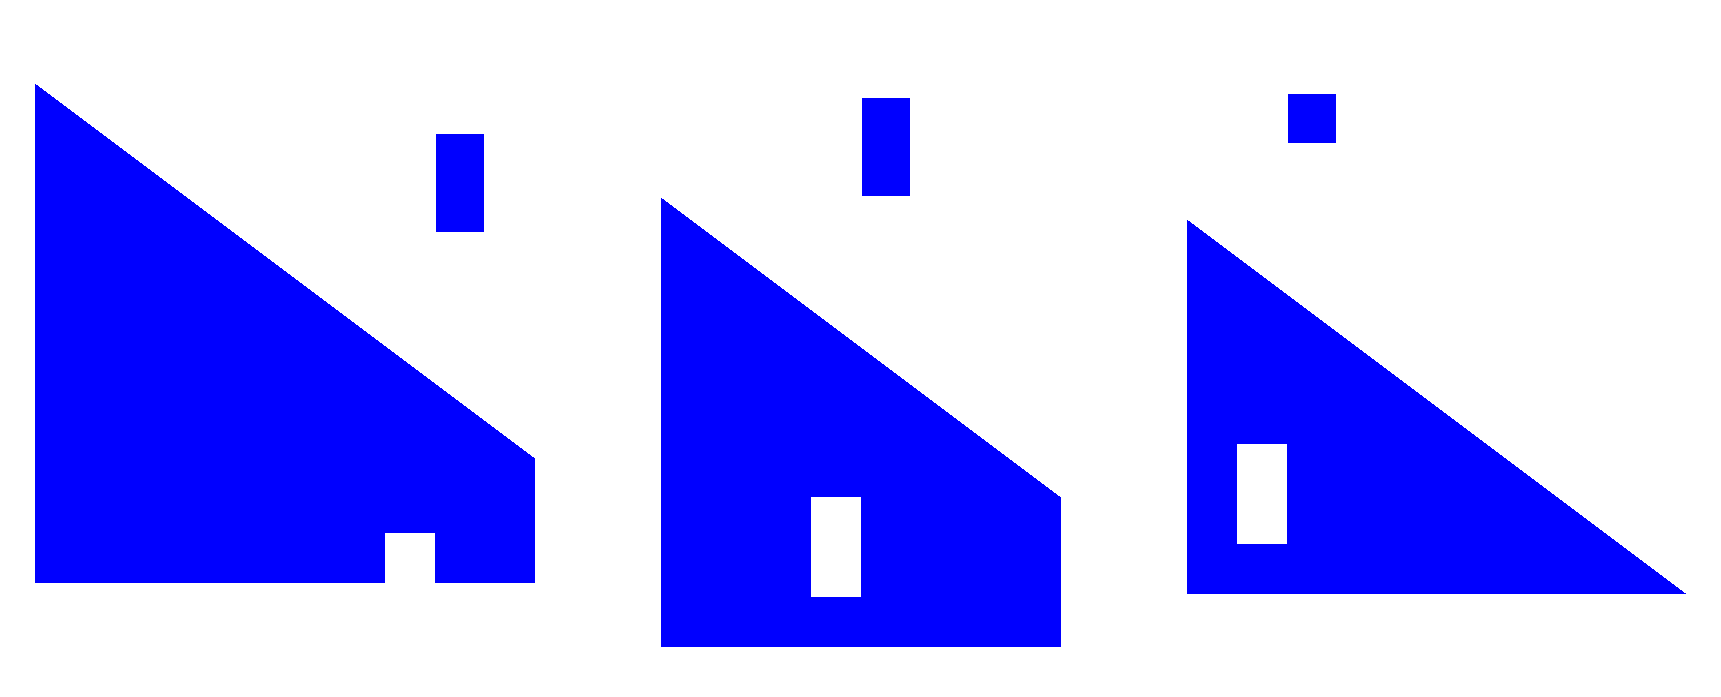
\includegraphics[width=0.9\linewidth]{pure_color}
    \end{center}
    \caption{Images with pure colors.}
    \label{fig:pc}
\end{figure}


\section{Testing}
% non-free SIFT
By default, the latest OpenCV's ``Stitcher'' class uses speeded up robust features (SURF) \cite{surf} to generate the feature,
rather than SIFT which is selected by Brown and Lowe's method.
However, the source code of SIFT feature extraction method is not included in the latest OpenCV.
The reason from the official \cite{cvcontri} is that SIFT method is a commercial method, and it is not free to use.

As well, I spent plenty of (wrong) time on dealing with Java Binding for the ``Stitcher'' class,
because by default the stitching class is not included in official Java binding class.
If I have to change the OpenCV methods, I have to write it in C++.
% todo: add some more information
So, if I have more time after writing the reports, I could be able to add more codes to implement the SIFT method and KNN matching method.

For metric test, I came up with two types of tests: quality test and performance test.
The quality test will evaluate the quality of resulting panorama, whereas the performance test will measure the statistical information while runnning.

\subsection{Quality Test}
At the beginning, I tried to experiment in a measurable way, which can produce some mathematical benchmark results. Here are the steps:
\begin{enumerate}
    \item Select a long image, \textit{(produce the images from panorama.)}
    \item Draw a horizontal line with 2 pixel width from left most to right most in vertical center, \textit{(create a baseline for benchmark, but the line should not affect the extracted feature set of the original images.)}
    \item \label{bm:sp} Split the image into three images: left, middle and right (each adjacent two images have 30\% shared area, and have same width), \textit{(make it simple, use only three images.)}
    \item Distort the left image to make the length of its left edge is two times larger than the length of its right edge, \textit{(simulate the projection effect.)}
    \item Distort the right image to make the length of its right edge is two times large than the length of its left edge, \textit{(simulate the projection effect.)}
    \item Rotate the left image for 30\degree clockwise, \textit{(just a random value to test , because ideally, the feature matching algorithm can match SIFT feature in any orientation.)}
    \item \label{bm:zoom} Zoom out to fit the rectangle window, \textit{(the image should still be a rectangle.)}
    \item Stitch them with Brown and Lowe's methods, \textit{(do stitching.)}
    \item Measure the following values, \textit{(benchmark.)} 
    \begin{itemize}
        \item The average running time with 30 repeats in millisecond,
        \item The mean square error (MSE) of the baseline's curvity,
        \item The minimum distance between each two baselines' endpoints in pixel,
              which is larger than 0 if the three baseline segments (each image has one) are not stitched together,
        \item The average image difference between the original long image and resulting image.
              This can be finished by patching Brown and Lowe's algorithm. After bundle adjustment, the image will be applied a gain compensation.
              After the gain compensation step, calculate the summary of RGB difference between the ``before'' image and ``after'' images.
    \end{itemize}
\end{enumerate}

However, the OpenCV implementation doesn't work on the benchmark method above, because there are not enough features matched evaluated by the probabilistic model.

One defect in the benchmark method is, the shared area selected in Step \ref{bm:sp} is too small to be kept in Step \ref{bm:zoom}.

Another defect of the benchmark method is as shown in Fig \ref{fig:fail}.
If the distortion in Step \ref{bm:zoom} is very arbitrary, the features sometimes cannot be detected successfully.
(The reason why I chose screenshot was that it could contain more useful features and less distracted features than normal images).

\begin{figure}[t]
    \begin{center}
        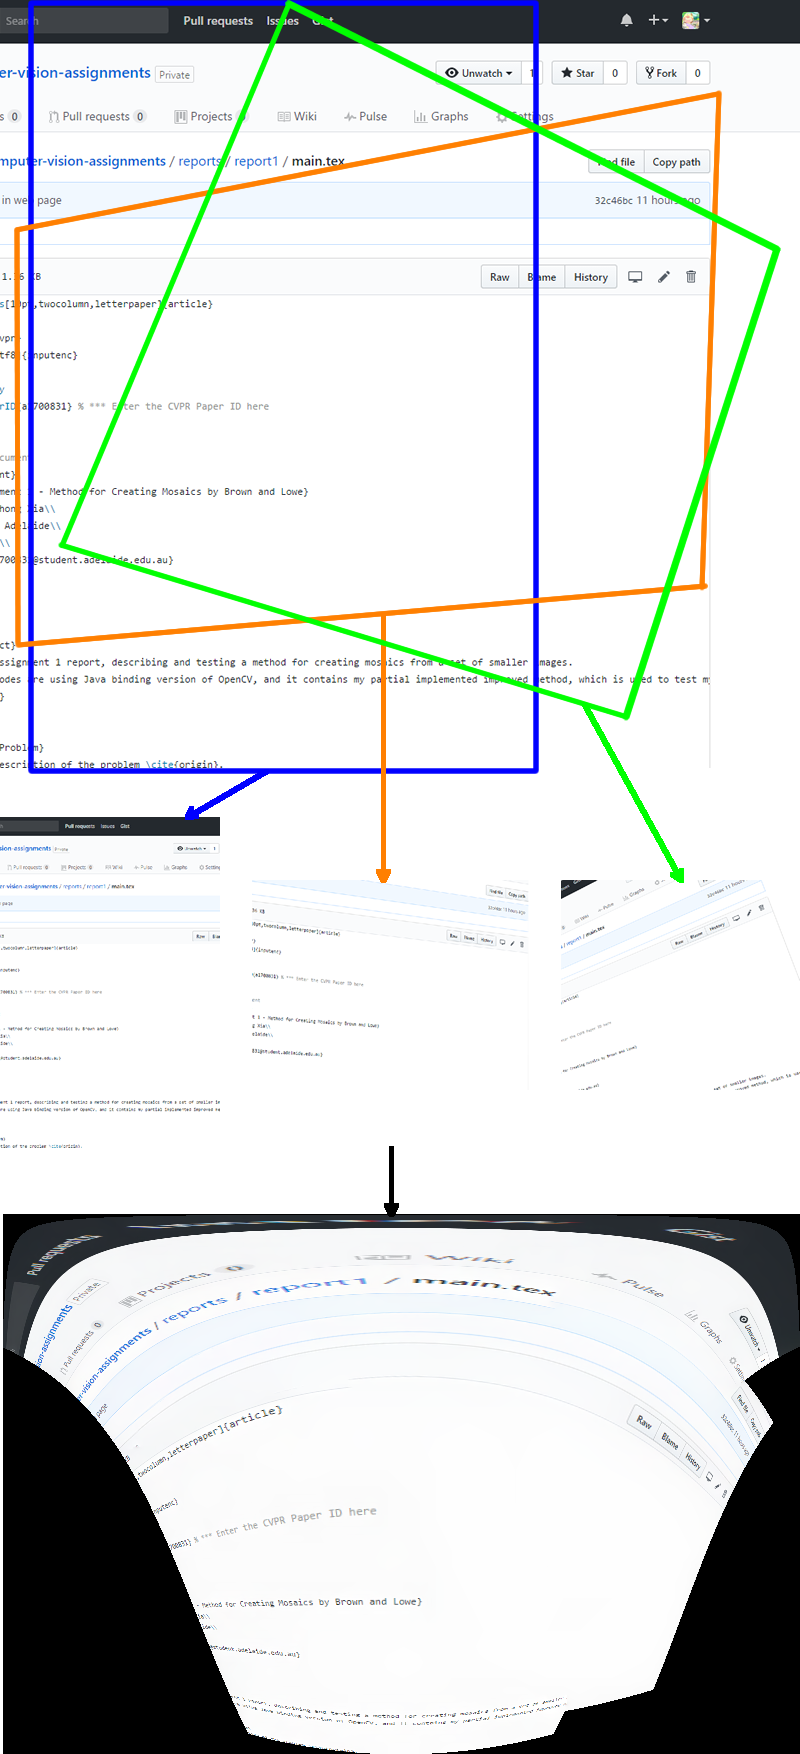
\includegraphics[width=0.9\linewidth]{fail}
    \end{center}
    \caption{The source image is a screenshot (plane), and the 3 images for stitching are cropped from the source image.
    Even when I tried using images with more than 70\% shared area, the result is still out of expectation.}
    \label{fig:fail}
\end{figure}

Thus, the quality test requires a simple single-variable controlled experiment.
The images should be as simpler as possible, and the number of features should be as larger as possible.

\subsection{Performance Test}
Performance is often evaluated by the time complexity and space complexity.
However, by following the methods from the paper, it is not available for evaluating its complexities,
because each step can be optimized by mathematical algorithms. 
As well, for the OpenCV implementation, the complexities are decided by the implementation of its data structures.
Therefore, the performance is not easy to be expressed by time or space complexities in this case.

\subsection{Method Attack and Test Conclusion}
The required testing will be finished by passing attacking photos.

I mentioned some weaknesses of Brown and Lowe's methods in Section 2.2,
and I have already attacked the method in Section 2.2, the 3rd point (Fig \ref{fig:cameramotion}).
It caused the method unable to find features.

As well in Section 2.2 the 2nd point, mult-band blending is easily affected by big moving objects.
If I produce two images with big objects in different position in each image, the resulting image will contain half, one, one and a half and two this objects.

Similarly, Fig \ref{fig:pc} also show the weakness and solutions to the probabilistic model for verifying images matching.
It just doesn't work for simple images because the method is trying to simulating a wider view len, and simple images is not considered to be likely to appear.
However, the method can be improved by patching Brown and Lowe's method, which is already discussed in Section 2.2.

Then I would like to perform some numeric testings.
In any feature extraction method, the most obvious attack is to add (more than 20\%) heavy noises into the graph.
The more features are extracted, the longer time the algorithm takes, because each feature will be tested in feature matching and image matching.
The results are shown on the table.

\begin{table}
\begin{center}
\begin{tabular}{|l|c|c|c|}
\hline
Image folder & Max & Min & Average \\
\hline\hline
Yosemite & 2078 & 1124 & 1465 \\
Yosemite\_noise & 3210 & 2338 & 2583 \\
Increased by & 54.48\% & 108.00\% & 76.30\% \\
\hline
\end{tabular}
\end{center}
\caption{Numeric comparison for adding new noises (images are stored in rc/yosemite\_noise). The noises are added online \cite{noise}, and arguments are: 50 noises, 50 strength. Each set of images are calculated by 30 repeats.}
\label{t1}
\end{table}

As is shown in the Table \ref{t1}, after adding noises, the calculation time is significantly increased.
And the noises affect the running time of both SIFT and SURF feature extraction methods.
As a result, Brown and Lowe's method is very robust because the added noises images can still be stitched together,
but the performance is very sensitive to the number of noises because it is determined by the invariant feature based idea.


% Bibliography
\begin{thebibliography}{9}
\bibitem {origin}
M. Brown and D. Lowe, ``Automatic panoramic image stitching using invariant features,''
\textit{Int. J. Comput. Vision}, vol. 74, no. 1, pp. 59–73, 2007.

\bibitem {sift}
D. G. Lowe, ``Distinctive Image Features from Scale-Invariant Keypoints,''
\textit{International Journal of Computer Vision}, vol. 60, 2004.

\bibitem {knn}
Beis, J. and Lowe, D. 1997. ``Shape indexing using approximate nearest neighbor search in high-dimensional spaces,''
\textit{In Proceedings of the Interational Conference on Computer Vision and Pattern Recognition (CVPR97)}, pp. 1000–1006.

\bibitem {ransac}
Fischler, M. and Bolles, R. 1981. Random sample consensus: ``A paradigm for model fitting with application to image analysis and automated cartography'',
\textit{Communications of the ACM}, 24:381–395.

\bibitem {bm}
Triggs, W., McLauchlan, P., Hartley, R., and Fitzgibbon, A. 1999. ``Bundle adjustment: A modern synthesis,''
\textit{In Vision Algorithms: Theory and Practice}, number 1883 in LNCS. Springer-Verlag. Corfu, Greece, pp. 298–373.

\bibitem {bascle}
Bascle, B., Blake, A., and Zisserman, A. 1996. ``Motion deblurring and super-resolution from and image sequence,''
\textit{In Proceedings of the 4th European Conference on Computer Vision (ECCV96)}. Springer-Verlag, pp. 312–320.

\bibitem {surf}
H., Bay, T., Tuytelaars and L., Van Gool, ``Surf: Speeded up robust features,''
\textit{Lecture Notes in Computer Science}, Vol.3951, p.404, 2006.

\bibitem {cvcontri}
OpenCV / opencv\_contrib: Repository for OpenCV's extra modules,
\textit{https://github.com/opencv/opencv\_contrib}

\bibitem {noise}
Add noise online,
\textit{http://pinetools.com/add-noise-image}

\end{thebibliography}

\end{document}
